As can be seen from fig. \ref{fig:loc1} localization depends on temperature: for the system under consideration, low-energy states are localized first, and then the middle of the spectrum (the area highlighted in blue in fig. \ref{fig:loc1}). The article \cite{pal_many-body_2010} specifically examines the occurrence of localization at $\beta=0$, that is, when in a thermal state all states are equally probable (however, for purity, all metrics will be calculated in the middle third of the spectrum). The system is considered to be a Heisenberg chain with random fields along the $z$-direction
\begin{equation*}
\hat{H} = J \sum_{j=1}^L \hat{\vc{S}}_j \cdot \hat{\vc{S}}_{j+1} + \sum_{j=1 }^L h_j \hat{S}_j^z,
\end{equation*}
for zero total spin, which is generally almost equivalent to the Hubbard hard-boson model and $h_j \in [-h,h]$. A phase transition is detected in the system at (or crossover?) at $h = h_c = \left(3.5 \pm 1\right)J$. The system is quite exotic in that we see a quantum phase transition at a non-zero temperature, and even in one dimension. To a large extent, this is possible precisely due to the lack of ergodicity in the system. 

The article performs Exact Diagonalization (ED) for $J=8,10,\ldots,16$. A phase transition is detected (fig. \ref{fig:metrics}a) by the already familiar $r$-parameter \eqref{eq:rparam}. Also, for all results, averaging is carried out over noise realizations.

It is also proposed to consider the decay of the longest wavelength disturbance of the spin density
\begin{equation*}
	\hat{M} = \sum_j \hat{S}_j^z \exp\left(i \frac{2\pi j}{L}\right).
\end{equation*}
Consider an initial condition that is at infinite temperature, but with a small modulation of the spin density in this mode, so the initial density matrix is $\rho_0 = (\1 + \epsilon \hat{M}\D) / Z$. For such an initial condition $\langle \hat{M}\rangle_0 = \tr (\rho_0 \hat{M})$. The long-time average of the spin polarization in this mode is
\begin{equation*}
	\langle \hat{M}\rangle_t = \frac{\epsilon}{Z} \sum_n \bk{n}[\hat{M}\D]{n} \bk{n}[\hat{M}\D]{n}.
\end{equation*}
They define the fraction of the contribution to the initial polarization that is dynamic and thus decays away (on average) at long time, as
\begin{equation*}
	f^{(n)} = 1 - \frac{\bk{n}[\hat{M}\D]{n} \bk{n}[\hat{M}\D]{n}}{\bk{n}[\hat{M}\D \hat{M}]{n} }.
\end{equation*}
In the ergodic phase, the system does thermalize, so the initial polarization does relax away and $f \to 1$. In the localized phase, on the other hand, there is no long-distance spin transport, so $f \to 0$. Это и наблюдается (fig. \ref{fig:metrics}a).


\begin{figure}[h]
    \centering
    \addletter{50}{a}
    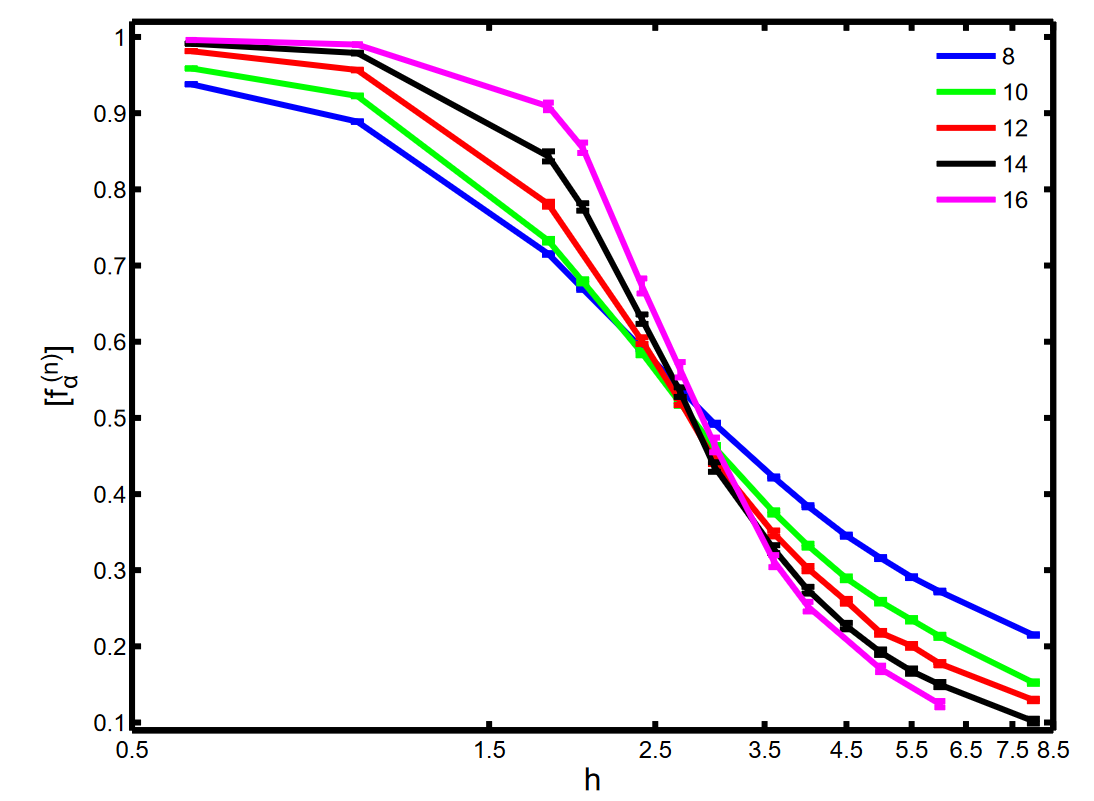
\includegraphics[align=c, width=0.3\textwidth]{imgs/metrics.png}
    \addletter{50}{b}
    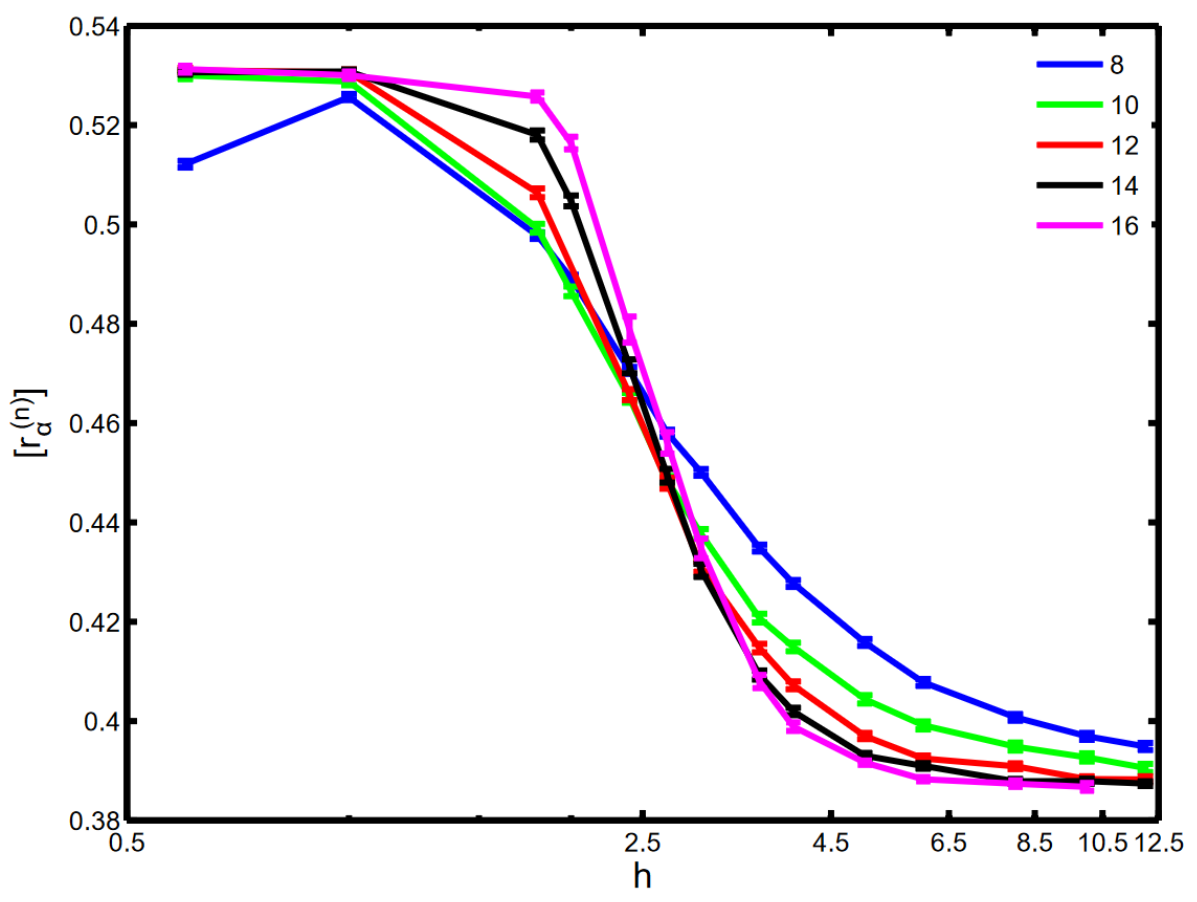
\includegraphics[align=c, width=0.3\textwidth]{imgs/metrics2.png}
    \addletter{50}{c}
    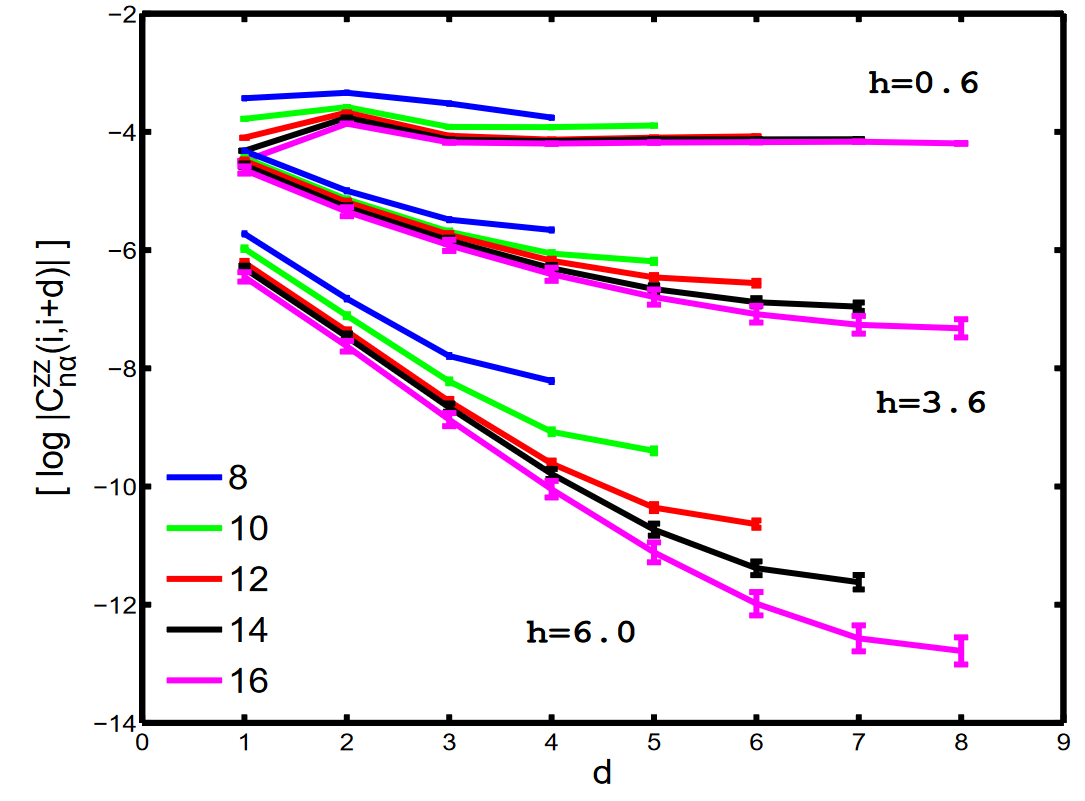
\includegraphics[align=c, width=0.3\textwidth]{imgs/metrics3.png}
    \caption{\cite{pal_many-body_2010} 
    a) The fraction of the initial spin polarization that is dynamic.
    b) The ratio of adjacent energy gaps ($r$-parameter).
    c) The spin-spin correlations in the manybody eigenstates as a function of the distance $d$.
    }
    \label{fig:metrics}
\end{figure}


Another way to detect a phase transition is to see that for large noises the correlations begin to decay exponentially
\begin{equation*}
C_n(i,j) = \bk{n}[\hat{S}^{i}_{z} \hat{S}^{j}_{z}]{n} - \bk{n}[ \hat{S}^{i}_{z} ]{n} \bk{n}[\hat{S}_j^z]{n},
\end{equation*}
where the average value $\langle \log |C_n(i,i+d)|\rangle_{i, n, h_j}$ is displayed (fig. \ref{fig:metrics}c).